\documentclass[11pt,a4paper]{report}
\usepackage[utf8]{inputenc}
\usepackage[francais]{babel}
\usepackage[T1]{fontenc}
\usepackage{amsmath}
\usepackage{amsfonts}
\usepackage{amssymb}
\usepackage{graphicx}
\usepackage{lmodern}
\usepackage{xlop}
\usepackage{minted}    
\usepackage[top=1cm, bottom=1cm, left=1cm, right=1cm]{geometry}
\author{Sylvain Julmy}
\newcommand{\z}{\mathbb{Z}}
\newcommand{\f}{\mathbb{F}}

% Python
\newminted{python}{frame=single, framesep=6pt, breaklines=true, fontsize=\scriptsize}
\newmintedfile{python}{frame=single, framesep=6pt, breaklines=true, fontsize=\scriptsize}

\begin{document}
\pagenumbering{gobble}
\paragraph*{Distance de hamming :} $d_h(x,y)$ nombre de composantes ou $x$ et $y$ diffèrent. $d_h(x,y) \leq d_h(x,z) + d_h(z,y)$.

\paragraph*{Code parfait :} Un code est dit parfait si les boules (disjointes) de rayon $\lfloor\frac{d-1}{2}\rfloor$ centrées aux mots du code recouvrent l'ensemble des mots. Par exemple, le code $\{(0,0,0,0,0),(1,1,1,1,1)\},$ est parfais tous les mots sont recouvert par les boules (on sait à partir de n'importe quel mot retrouver son mot du code le plus proche), avec le même code mais une répétition de $4$ ce n'est plus le cas, si on reçoit $(0,0,1,1)$ on ne sais pas à quel mot du code il appartient. 

\paragraph*{Code en bloc :}$n$ est la longueur du code. $c$ est émis et $r$ est reçus. Code à simple contrôle de parité : somme des bits pairs (impair -> 1, pair -> 0). Détecte $1$ erreur mais pas $2$ ($d=2$). Ne corrige aucune erreur. Code à répétition : (pour $repet=4$, $4$ répétition du même bit) détecte $4$ erreurs et corrige $2$ erreurs ($d=5$). $d$ est la distance minimal entre deux mots différents du code. Un code en bloc détecte $d-1$ erreurs et corrige $\frac{d-1}{2}$ (arrondis inférieur) erreurs. Une boule de rayon $d-1$ centré sur un mot du code ne contient pas d'autre mot du code (si centré en $d$ alors au moins $1$ mot du code).

\paragraph*{Nombre premier :} un nombre est premier seulement si il est divisible par $1$ et par lui-même. Le nombre de nombre premier entre $1$ et $n$ est donné par la formule $\pi(n)\approx\frac{1}{\ln(x)}$ (pas pareil que $\phi(n)$ !). Si $p$ premier, $\phi(p)=p-1$. Si $p \neq q$ premiers alors $\phi(pq)=(p-1)(q-1)$.

\paragraph*{Petit théorème de Fermat :} si $p$ premier, $pgcd(a,p)=1 \rightarrow a^{\phi(p)} = a^{p-1} \equiv 1 \mod p$ et $a^p \equiv a \mod p$. Par contre, si on ne sait pas si $p$ est premier ou non, on ne peut pas dire que $p$ est composé si $a^n\approx a\mod n$. Il existe des nombres (de Carmichaël) qui ont cette propriété (par exemple $561=3\cdot11\cdot17$).

\paragraph*{Division euclidienne :} $\frac{14}{5} = 2\cdot5+4 \rightarrow a=qb+r,\ r=a\mod b$. Tout nombre est un facteur unique de nombres premiers. Pour trouver un nombre premier : crible d'Érathosthène (tester jusqu'à $t\geq\sqrt{n}$). Infinité de nombre premier, $\pi(x)\approx\frac{1}{\ln(x)}$.

\paragraph*{PGCD :} Plus grand commun diviseur, $ppcm(a,b)$ plus petit commun multiple. $pgcd(a,b)\cdot ppcm(a,b) = a\cdot b\ \forall a,b > 0$. $pgcd(a,b) = pgcd(b,a\mod b)$. Pour calculer le PPCM, il suffit de calculer $\frac{a\cdot b}{pgcd(a,b)}$.

\paragraph*{Euclide étendu :} $pgcd(a,b)=ua+vb$ : démarrer avec $r_1=a,r_2=b,q_1=\emptyset,u_1=1,u_2=0,v_1=0,v_2=1$. Ensuite, répéter tant que $r\neq0$ :

\begin{minipage}{0.45\textwidth}
\begin{itemize}
    \item $r_i = r_{i-2} \mod r_{i-1}$
    \item $q_{i-1} = r_{i-2} \div r_{i-1}$ (division euclidienne)
    \item $u_i=u_{i-1}\cdot -q_{i-1} + u_{i-1}$
    \item $v_i=v_{i-1}\cdot -q_{i-1} + v_{i-1}$
\end{itemize}
\end{minipage}
\begin{minipage}{0.45\textwidth}
\begin{itemize}
    \item $pgcd(a,b)=ua+bv$
    \item $m\cdot pgcd(a,b)=m\cdot ua+m\cdot bv$
    \item $sa+tb=s\alpha pgcd(a,b)+t\beta pgcd(a,b) = (s\alpha+t\beta)pgcd(a,b)$
    \item Un multiple entier de $pgcd(a,b)$ est une combinaison linéaire de $a$ et $b$
\end{itemize}
\end{minipage}

\paragraph*{Congruence modulo $m$ :} $m\in \mathbb{N}, m \geq 1,{a,b}\in \mathbb{Z}$. $a$ congru à $b$ modulo $m$ : $a\equiv b \mod m \rightarrow a\mod m = b\mod m$,$a-b\mod m = 0$ $a=b+km,k\in \mathbb{Z}$. 
\begin{itemize}
    \item $a\equiv b \mod m,c\equiv d \mod m \rightarrow -a \equiv -b \mod m, a+c \equiv b+d \mod m, ac \equiv bd \mod m$
    \item $ab \equiv ac \mod m \wedge pgcd(a,m)=1 \rightarrow b \equiv c \mod m$
    \item $a \equiv b \mod m \wedge a \equiv b \mod n \rightarrow a \equiv b \mod mn$
\end{itemize}

\paragraph*{Inverse modulo $m$ :} Calculer l'inverse de $a$ modulo $m$ : Euclide étendue $\rightarrow ua+vm=1$, $u$ est l'inverse modulo $m$ de $a$.

\paragraph*{Indicatrice de Euler :} $\phi(n)$ nombre de nombre premier avec $n$. Si $p$ premier, alors $\phi(p)=p-1$, si $p\neq q$ premiers, alors $\phi(pq)=(p-1)(q-1)$.

\paragraph*{Thèorème d'Euler :} $a\in\mathbb{Z},m\geq1,pgcd(a,m)=1 \rightarrow a^{\phi(m)} \equiv 1 \mod m$. $a^{\phi(m)-1}$ est donc l'inverse de $a$ modulo $m$ si $a$ est premier à $m$.

\paragraph*{RSA :} Choisir $p$ et $q$ premiers. $n=pq$, $\phi(n)=(p-1)(q-1)$, choisir $e$ premier à $\phi(n)$ et $e<\phi(n)$ ($pgcd(e,\phi(n))=1$, calculer $d$ comme l'inverse de $e$ modulo $\phi(n)$ avec Euclide étendu. Clé publique : $(n,e)$, clé privé : $(n,d)$. Chiffre un message $M$ : $C = M^e \mod n$. Déchiffrer un message : $M = C^d\mod n$.

\paragraph*{Théorème des restes chinois :} Résoudre le système $x \equiv a_1 \mod a_2, x \equiv b_1 \mod b_2, x \equiv c_1 \mod c_2$. $\bowtie(a,b,c)$ est l'inverse de $ab$ modulo $c$. $x = a_1 \cdot \bowtie(b_2,c_2,a_2) \cdot b_2c_2 + b_1 \cdot \bowtie(a_2,c_2,b_2) \cdot a_2c_2 + c_1 \cdot \bowtie(a_2,b_2,c_2) \cdot a_2b_2$

\paragraph*{Anneau $\mathbb{Z}/\mathbb{Z}$ :} $m\in\mathbb{N}^*$,$\z/m\z=\z/m=\{0,1,...,m-1\}$,$0=m=-m=2m=...$. Addition et multiplication change pas. Tous les éléments (différent de $0$) on un inverse modulo $m$ (Euclide étendue). Règle de calcul usuel (associativité,...). $m\cdot a = 0$.

\paragraph*{Anneau $\z/p\z$, $p$ premier :} $a^{\phi(p)}=a^{p-1}=1 \forall a \in (\z/p\z)^*$. Ordre de $a\in(\z/p\z)^*$ plus petit exposant entier $e$ tel que $e\geq1$ et $a^e=1$, l'ordre de $a$ divise toujours $p-2$. Ordre de $a^l = ppcm(l,e_a)/pgcd(e_a,l)$ et divise donc l'ordre de $a$. Il existe toujours un élément $\alpha$ dont les puissances successives engendre tous les éléments du corps. Un corps fini compte $p^\nu$ éléments avec $p$ premier. Il existe $\phi(p-1)$ générateurs. Si $\alpha$ est générateur : $a^l$ générateur si et seulement si $l\in{1,2,...,p-1}$ premier à $p-1$. \textbf{Pour construire les tables : faire addition + multiplication le tout modulo $p$}.

\paragraph*{Éléments inversibles d'un corps :} tous les éléments, sauf $0$, sont inversibles dans un corps.

\paragraph*{Savoir si un polynôme est irréductible dans $\f_2$ :} Est-ce qu'il s'annule pour $0$ ou $1$ ? Est-ce qu'il est carré d'un polynôme (racine impair -> non) ? Divisible par $x^2+x+1$ ? Dans $\mathbb{C}$ il n'existe pas de polynôme irréductible de degré $\geq 1$.\\
\textbf{Pour trouver les polynômes irréductibles}, partir des polynômes de degrés $1$ et calculer les suivants. Il ne doivent s'annuler ni en $0$ ni en $1$ donc le terme constant vaut $1$ et il doit y avoir un nombre impair de termes.

\paragraph*{Structure additive de $\mathbb{F}_{p^\nu}$ :} Ensemble des vecteurs $a=(a_0,a_1,...,a_{\nu-1})$ à $\nu$ composantes. $a+b$ : addition composante par composante. $\lambda a$ : multiplication de chaque composante par $\lambda$. $a=(a_0,a_1,...,a_{\nu-1}=a_0+a_1x+a_2x^2+...+a_{\nu-1}x^{\nu-1}=a(x)$.

\paragraph*{Table d'addition et multiplication dans $\f_{2^\nu}$ :} Addition composante par composante avec un XOR. Donc la diagonale vaut $0$. Les éléments sont des vecteurs de longueur $\nu$. Dans $\f_{2^3}^*$ tous les éléments sont générateurs, on obtient donc $x=2,x^3=3,x^2=4,x^6=5,x^4=6,x^5=7$ codé en binaire. Ensuite, pour l'addition, on utilise la formule $x^kx^l=x^{k+l}$. On a $m(x)=x^3+x+1$, donc $x^3=x+1=2+1=3$. On construit les puissances des colonnes et des lignes à partir de $0$, $1$, $x$ et $m(x)$.

\paragraph*{$F[x]$ :} Ensemble des polynômes en $x$ à coefficient $\in F$. $a(x_0)=0$. Des polynômes différents peuvent être égales sur $F$. $a(x) = q(x)b(x)+r(x)$ (division euclidienne). $r(x) = a(x) \mod b(x)$. Tout polynôme de $F$ est un produit unique de $\alpha\in F$ et de polynôme unitaires irréductibles. $x^2+x+1\in F[x]$ seul polynôme irréductible de degré $2$. Pour le $pgcd(a(x),b(x)$ ne change pas de la façon normale. La congruence ne change pas de la congruence dans $\z$.

\paragraph*{Exemple $\mathbb{F}_4 = \mathbb{F}_{2^2}$ :} $x^2+x+1$ est irréductible, on a donc $x^2=x+1$. Donc $x\cdot x = x^2 = x+1$.

\paragraph*{Code linéaire :} $F=\mathbb{F}_{p^\nu}$, souvent $\mathbb{F}_2$. $n$ est la longueur du code, $k$ la dimension. Pour un mot $x$, $w(x)$ est le poids du mot (nombre de composante non-nulle), $d_h(x,y) = w(x-y)$. Un code est linéaire si les mots s'exprime sous la forme $c=aG$.

\paragraph*{Exemple :} $C=\{0000,1011,0110,1101\}$, $k=2$ ($0$ ou $1$),$n=4$,$d=w_{min}=w(0110)=2$. Code de type $(n=4,k=2,d=2)$. Matrice génératrice : $[1011;0110]$. La matrice est systématique si elle contient une sous-matrice unitaire. Si une matrice n'est pas systématique : transformation par l'algorithme de Gauss.

\paragraph*{Code engendrer par des vecteurs :} On à $b_0$ et $b_1$ comme vecteur, on a donc un code avec $\{0,b_0,b_1,b_0+b_1\}$ (addition avec un XOR). La matrice $G$ est créer avec ces vecteurs, essayer d'avoir une matrice systématique avec par exemple $G=[b_0;b_0+b_1]$.

\paragraph*{Matrice systématique :} Pour simple contrôle de parité : $G$ est une matrice identité avec une colonne de $1$. Pour un code à répétition, $G$ est un vecteur de longueur $n$ de $1$.

\paragraph*{Produit scalaire de polynôme :} $x=(x_0,...,x_{n-1}), y=(y_0,...,y_{n-1}) \in F^n$, $\langle x,y\rangle = xy^T=\sum_{l=0}^{n-1}x_l y_l$. Les mots d'un code linéaire sont caractériser par les mots auxquels ils sont tous perpendiculaires.

\paragraph*{Code dual :} Si $G$ est une matrice génératrice et $G=(I_k|P)$ systématique, alors $H=(-P^T|I_{n-k})$ matrice génératrice de $C^T$. $GH^T=O$ car lignes de $G$ perpendiculaire à lignes de $H$. $x\in F^n$, $H$ matrice de contrôle de $C$ : $x\in X \leftrightarrow xH^T = 0 \in F^{n-k}$. Un code est de type $(n,k,d)$.\textbf{Pour déterminer le code $C$ à partir de $G$ : ajouter $0$ et addition des deux vecteurs de $G$}.

\paragraph*{Syndrome :} $S(x) = xH^T$, $S(x)=0$ si $x$ est un mot du code. Mot $c$ du code émis : $r=c+e \rightarrow S(r)=S(c)+S(e)=S(e)$, ne dépend que de l'erreur ajoutée. Pour calculer le syndrome à partir de $H$, on commence par $0$, puis les colonnes de $h$ et pour finir on additionne les syndromes des en-têtes qui formes les en-têtes en dehors des mots du code. \textbf{Pour attribuer les syndromes, toujours commencer par l'en-tête avec le $1$ le plus à droite et seul}.

\paragraph*{Tableau standard :} $G=\begin{pmatrix}1&0&1&1\\0&1&1&0\end{pmatrix}, H=\begin{pmatrix}1&1&1&0\\1&0&0&1\end{pmatrix}$. Construction du tableau standard : 1ère ligne $\rightarrow$ mots du code en commençant par $0$. Ensuite, prendre un mot de poids minimal pour la tête de ligne et remplir le reste de la ligne avec un XOR à l'intersection. Pour décoder par le tableau standard : le mot reçus auquel on soustrait la tête de ligne. \textbf{Mots hors du code :} distance plus grandes que les boules de rayon souhaités (voir la première colonne). \textbf{Pour trouver $H$ :} à partir de $G$, prendre la partie non-systématique de $G$, la transposer et la mettre à droite dans $H$, remplir le reste avec une matrice identité. 

\paragraph*{Décodage par le syndrome :} Calculer les syndromes des têtes de lignes. Syndrome des têtes de lignes : $00$, $11$, $10$, $01$. On reçoit $r=1111$, on calcule le syndrome $rH^T=10$, tête de la troisième ligne : $1111 - 0100 = 1111 \oplus 0100 = 1011$. Code de type (4,2,2), ne corrige aucune erreur.

\paragraph*{Code de Hamming bianire :} $H=3,5,6,7,4,2,1$ écrits en binaire, $d=3$, $G=8,4,2,1,7,11,13$ écrits en binaire. C'est un code parfait : les boules disjointes de rayon $1$ centrées aux $2^4$ mots du code, à $8$ mots chacune, recouvrent bien les $2^4\cdot 8=2^7$ mots. Idem pour $H(8,4,4)$.

\paragraph*{Codes cycliques (Anneau $F[x]/(x^n-1)$) :} On considère des polynômes $u(x)\in F[x]/(x^n-1)$ : $u(x)=u(x)\mod(x^n-1)$, on a $x^n = 1, x^N=x^{N\mod n}$. Tout mot $\in F[x]/(x^n-1)$ est représenté par un polynôme de degré $<n$. $v(x)=v_0+v_1x+...+v_{n-2}x^{n-2}\in F[x]/(x^n-1)$, quand on multiplie par $x$ : $xv(x) = v_0x+v_1x^2+...+v_{n-2}x^{n-1}$, c'est donc un décalage circulaire des composantes de $v$ vers la droite.

\paragraph*{Simplification de polynômes :} Prendre les puissances du polynôme modulo la puissance de $m(x)$ dans $\f_2[x]/(x^n-1)$. Si deux fois la même puissance (par exemple $x^4 + x^4$, ça s'annule).

\paragraph*{Factorisation de $x^n-1$ dans $\f_\nu$ :} Trouver une racine, factoriser et recommencer jusqu'à n'avoir que des facteurs irréductibles. Exemple : $\nu=2$ $x^3-1=(x+1)(x^2+x+1)$.

\paragraph*{Matrice de contrôle d'un code cyclique (Exemple) :} Déterminer une matrice de contrôle du code cyclique ternaire de longueur $4$ engendré par $g(x)=x^2+1$ : $h(x)=(x^4-1)/(x^2+1)=x^2-1=x^2+2 \in \f_3[x]$. $H=\begin{pmatrix}1&0&2&0\\0&1&0&2\end{pmatrix}$. $d=2$ donc le code est de type $(4,2,2)$.

\paragraph*{Polynôme générateur du code :} $x^n-1 = (x-1)(...)$. On choisis un diviseur unitaire $g(x)$ de $x^n-1$ dans $F[x]$. On aura donc un contrôle avec $h(x)=(x^n-1)/g(x)$. Exemple pour $F=\mathbb{F}_2$,$n=7$ : $x^7-1 = (x-1)(x^3+x+1)(x^3+x^2+1)$, $g(x)=x^3+x+1$ et $h(x)=(x-1)(x^3+x^2+1)=x^4+x^2+x+1$. 

\paragraph*{Matrice génératrice :} Chaque mot du code est représenter par son reste modulo $x^n-1 \rightarrow a(x)g(x)\in F[x]/(x^n-1)$ pour un seul $a(x)=a_0+a_1x+...+a_{k-1}x^{k-1}\in F[x]$ de degré $< k = n-deg(g(x))$. $g(x) = g_0+g_1x+...+g_{n-k}x^{n-k}$ unitaire de degré $n-k$.
$G = \begin{pmatrix}
g_0 & g_1 & g_2 & ... & g_{n-k} & 0 & ... & ... & 0 \\
0   & g_0 & g_1 & g_2 & ... & g_{n-k} & 0 & ... & 0 \\
\vdots & \ddots & \ddots & \ddots & \ddots & \ddots & \ddots & \ddots & \vdots \\
0 & ... & 0 & g_0 & g_1 & g_2 & ... & g_{n-k} & 0 \\
0 & ... & ... & 0 & g_0 & g_1 & g_2 & ... & g_{n-k}
\end{pmatrix}$. $\textbf{c=aG}$\\\textbf{Exemple :} Code cyclique binaire de longueur $7$, $g(x)=1+x+x^3$, $h(x)=x^4+x^2+x+1$.\\$G=\begin{pmatrix}
1&1&0&1&0&0&0\\
0&1&1&0&1&0&0\\
0&0&1&1&0&1&0\\
0&0&0&1&1&0&1\\
\end{pmatrix}$, $H=\begin{pmatrix}
1&0&1&1&1&0&0\\
0&1&0&1&1&1&0\\
0&0&1&0&1&1&1
\end{pmatrix}$ : Hamming(7,4).

\paragraph*{Matrice génératrice systématique :} $g(x)=x^3+x+1$ dans $\mathbb{F}_2[x]/(x^7-1)$:

\begin{minipage}{0.45\textwidth}
\begin{itemize}
    \item $x^3=1\cdot g(x) + reste$
    \item $x^4=xg(x)+reste$
    \item $x^5=(x^2+1)g(x)+reste$
    \item $x^6=(x^3+x+1)g(x)+reste$
\end{itemize}
\end{minipage}
\begin{minipage}{0.45\textwidth}
$G_s=\begin{pmatrix}x^3\\x^4\\x^5\\x^6\end{pmatrix}=
\begin{pmatrix}
1&1&0&1&0&0&0\\
0&1&1&0&1&0&0\\
1&1&1&0&0&1&0\\
1&0&1&0&0&0&1
\end{pmatrix}$
\end{minipage}

\paragraph*{Polynôme syndrome :} $\sigma(v(x))=v(x)\mod g(x) \in F[x]$: reste de la division du mot $v(x)$ par $g(x)$. Si $\sigma(v(x))=0 \leftrightarrow v(x)\in C$. Ne dépend que du polynôme d'erreur ajouté lors de la transmission. Le décodage est correct si $r(x) \leq \lfloor\frac{d-1}{2}\rfloor$.

\paragraph*{Corps $\mathbb{F}_{2^\nu}$ (Exemple) :} $\nu=4$, polynôme irréductible primitif $m(x)=x^4+x+1\in \mathbb{F_2[x]}$ de degré $\nu$. $\f_{16}=\f_{2^4}=\f_2[x]/(m(x))$. $\alpha = x \in \f_{16}$ : $\f_{16} = \{0,\alpha,\alpha^2,...,\alpha^{15}=1\}$. $\f_{2^4}$ est un espace vectoriel de dimension $4$ sur $\f_2$ avec comme base $1,\alpha,\alpha^2,\alpha^3$. On peut coder $0,1,\alpha,\alpha^2,...,\alpha^{15}$ comme des combinaisons linéaires de $1,\alpha,\alpha^2,\alpha^3$. On a $m(x)=x^4+x+1$ donc $\alpha^4=1+\alpha$.

\paragraph*{Polynômes minimaux :} les polynômes minimaux sont les polynômes irréductibles d'un corps. Par exemple : $x^15-1 = (x-1)(x^4+x+1)(x^4+x^3+x^2+x+1)(x^2+x+1)(x^4+x^3+1)$. Le degré des polynômes minimaux est $\leq \nu$ : $(\alpha^l)^{2^\nu} = (\alpha^{2^\nu})^l=\alpha^l$.

\paragraph*{One-time pad :}

Soit un message $x$ de $l$ bits, on génère une clef de $l$ bits complètement aléatoire. On transmet la clef à Bob et on calcule le texte chiffré $y=x\oplus k$, où $\oplus$ est un XOR. Ce code est parfaitement sûr.

Un chiffrement est dit parfaitement sûr si le texte clair $x$ et le texte chiffré $y$ sont statistiquement indépendant:
$$ P[X|Y] = P[X] $$
Ce qui vaut
$$ P[X|Y] = \frac{P[X \wedge Y]}{P[Y]} $$

Inconvénient : clef unique, le texte chiffré peut être manipulé, la transmission des clefs posent problèmes et la génération d'une clef aléatoire est problématique.

\paragraph*{RC4 :}

RC4 n'est pas recommandé en pratique, on initialise une clé puis on utilise un générateur de flot pseudo-aléatoire en essayant de reproduire le "one-time pad".

\paragraph*{Grain :}

Algorithme qui prend une clef de 80 bits et un vecteur d'initialisation de 64 bits. Économe en ressource si implémenter sur FPGA et encore incassé à ce jour.

\begin{center}
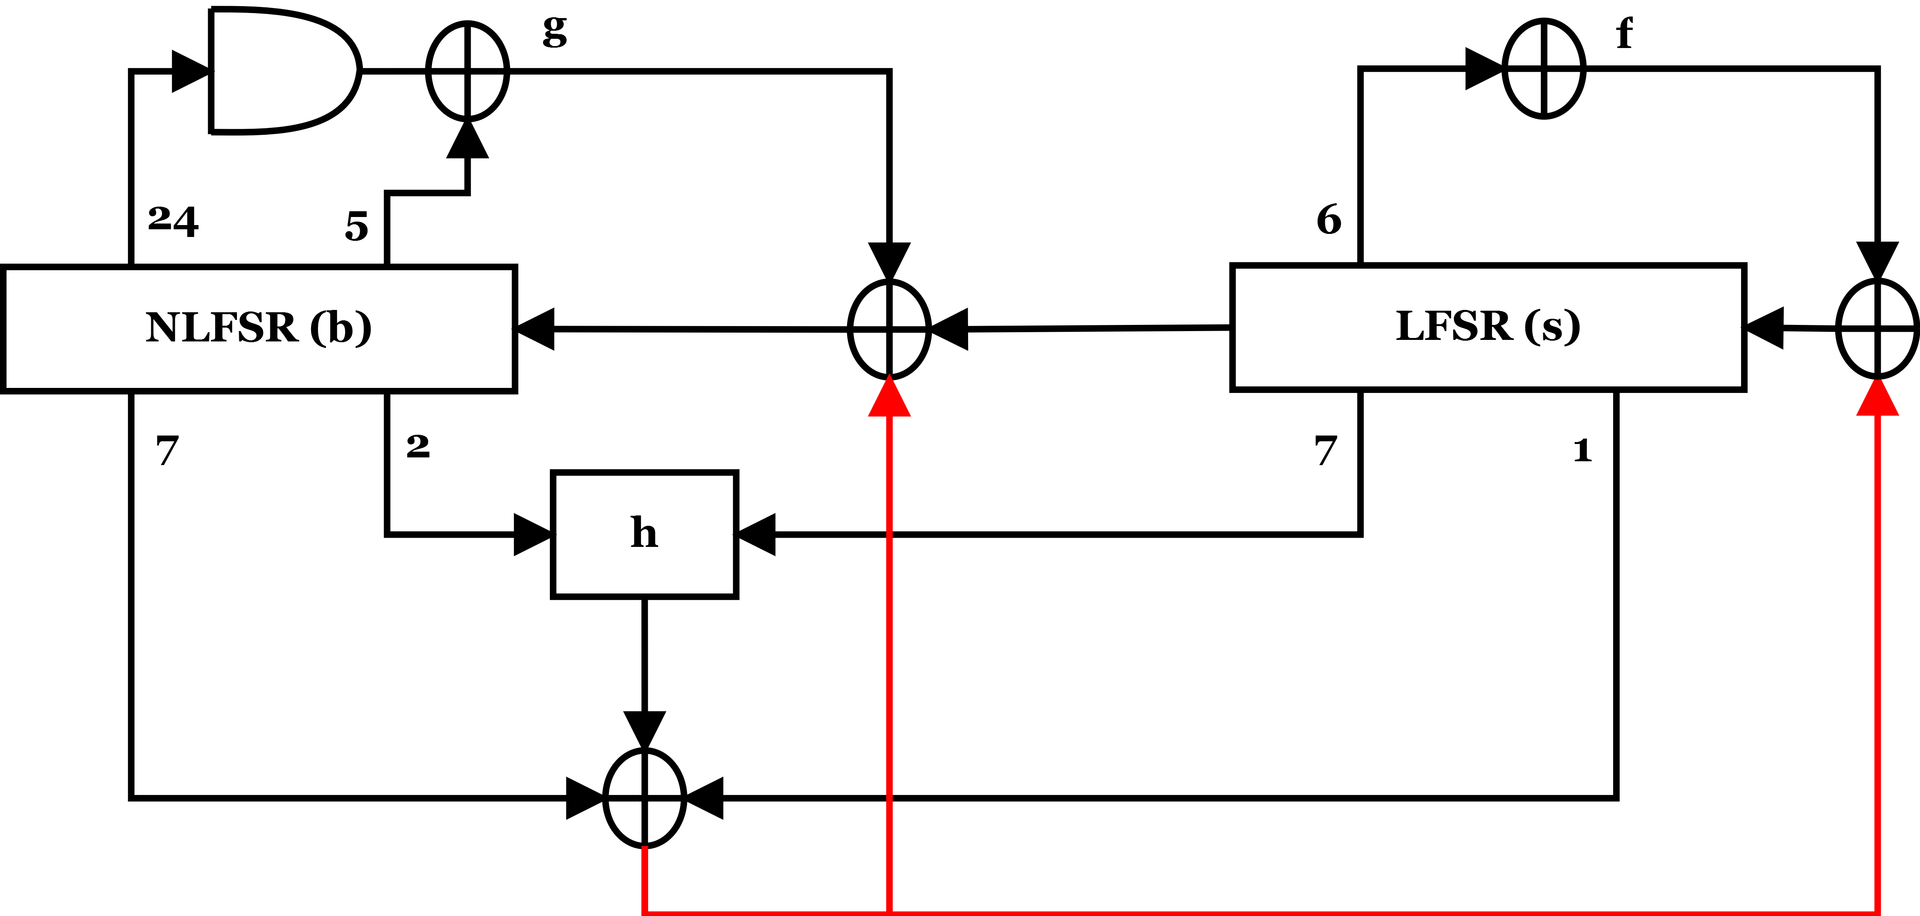
\includegraphics[width=0.5\textwidth]{img/Grain_init.png}
\end{center}

\paragraph*{Chiffrement par bloc :}

Étant donné un chiffrement par bloc $F$ qui chiffre des textes clairs $X = \{x_1,...,x_l\}$ de $l$ bits au moyen d'une clef $K$, où $x_i \in \mathbb{Z}_2$, on peut écrire $F$ sous la forme d'un système d'équations booléennes :
\begin{align*}
&y_1 = F^1_K(x_1,...,x_l) \\
&... \\
&y_l = F^l_K(x_1,...,x_l)
\end{align*}

Confusion : les fonctions $F^1_K,...,F^l_K$ doivent être mathématiquement complexes car en pratique on peut trouver la clef $K$ au moyen du texte clair et du texte chiffré. Les fonctions ne doivent pas être linéaire.

Diffusion : Une modification d'un seul bit du texte clair devrait changer en moyenne la moitié des bits du texte chiffré.

\paragraph*{Recherche exhaustive de clef :}

Le principe est d'essayer toutes les clefs possibles. La recherche exige un critère d'arrêt : comment savoir que la clef est bonne ? Pour une clef de $l$ bits, il faut au minimum $1$ essai, au pire des cas $2^l$ essais et en moyenne $2^{l-1}$ essais. En 2015, une taille de clef de $64$ bits est considéré comme insuffisante. $80$ bits en minimal. Moore : la puissance de calcule double environ tous les 18 mois.

\paragraph*{Chiffrement itéré :}

Itérer une fonction de ronde un certain nombre de fois. Chaque fonction de ronde prend comme paramètre un sous-clef de la clef principale au moyen de cadencement de clef. Le but est de trouver un équilibre entre nombre d'itération et force du code.

\paragraph*{DES}

Prend une clef de $64$ bits dont $8$ bits ignorés (donc $56$ bits) et est bâti sur un schéma de Feistel à $16$ rondes.

$IP$ est une matrice de permutation sur $\mathbb{Z}_2$ de taille $64 \times 64$ et $FP$ est son inverse. $E$ est une fonction linéaire qui étend son entrée de $32$ bits en une sortie de $48$ bits en dupliquant certains bits. $P$ est une matrice de permutation de $32 \times 32$. $PC1$ est une fonction linéaire qui passe de $64$ bits à $56$ bits. $PC2$ est une fonction linéaire qui passe de $56$ bits à $48$ bits

\paragraph*{Triple DES}

Triple DES à deux clefs  : $Y = DES_{K1}(DES_{K2}^{-1}(DES_{K1}(X)))$ \\
Triple DES à trois clefs : $Y = DES_{K3}(DES_{K2}^{-1}(DES_{K1}(X)))$

\paragraph*{IDEA}

Possède une clef de $128$ bits, sa fonction de ronde est itérée $8.5$ fois et qui chiffre des blocs de données de $64$ bits. IDEA repose sur l'utilisation de 3 opérations incompatibles algébriquement :
\begin{itemize}
    \item l'addition sur $\mathbb{Z}^{16}_2$ notée $\oplus$
    \item l'addition sur $\mathbb{Z}_{2^{16}}$ notée $\boxtimes$
    \item la multiplication sur $\mathbb{Z}_{2^{16}+1}$, notée $\odot$ et où $0$ est identifié à la valeur $2^{16}$.
\end{itemize}

IDEA est basé sur un schéma de Lai-Nassem.

\paragraph*{AES}

Chiffre des données de $128$ bits qui supporte des clefs de $128$ bits (10 rondes), $192$ bits (12 rondes) et $256$ bits (14 rondes). Très efficace sur les plateformes embarquées, CPU et hardware.

\paragraph*{Mode opératoire}

Un algorithme de chiffrement par flot peut chiffrer des données de n'importe quelle longueur contrairement à un algorithme de chiffrement par bloc (64 ou 128 bit typiquement).

Un mode opératoire est une manière de chiffrer des données plus grandes que la taille d'un bloc. Modes classiques :
\begin{itemize}
    \item "Electronic Code Block" ECB
    \item "Cipher Block Chaining" CBC
    \item "Counter Mode" CTR
    \item CFB, OFB,...
\end{itemize}

\paragraph*{ECB}

Les données à chiffrer sont divisées en blocs de la taille du bloc de l'algorithme de chiffrement, chaque bloc est chiffré indépendamment des autres.

\paragraph*{Problème : } Deux blocs de textes clairs identiques seront chiffrés de manières identiques. On a donc une perte potentielle de confidentialité. Le mode ECB résiste donc très mal aux attaques visant à modifier l'intégrité du texte chiffré. C'est un algorithme déterministe.

\paragraph*{CBC}

\paragraph*{Principe : }
\begin{itemize}
    \item les données sont divisées en blocs de la taille du bloc de l'algorithme de chiffrement
    \item avant le chiffrement, un bloc est combiné avec un XOR avec le texte chiffré précédent
    \item Le premier bloc est combiné avec un bloc de chiffrement aléatoire appelé \textbf{vecteur d'initialisation} (IV)
\end{itemize}

Chaque bloc de texte chiffré est dépendant de tous les blocs précédents. Le chiffrement est séquentiel mais le déchiffrement peut être parallèle.

\paragraph*{CTR}

\begin{itemize}
    \item Un compteur est chiffré par l'algorithme de chiffrement par bloc
    \item Le flux est combiné au moyen d'un XOR avec le texte clair
\end{itemize}

Algorithme parallèle, pas besoin de couper des données si pas de la bonne taille, la sécurité repose sur la qualité de l'IV, mauvaise résistance aux adversaires attaquant l'intégrité du texte chiffré.

\paragraph*{Fonction de hachage}

Fonction définis comme $H:\{0,1\}* \rightarrow \{0,1\}^l$ qui possède les propriétés suivantes :
\begin{itemize}
    \item le calcul de l'empreinte (digest) $h = H(m)$ d'une message $m$ est une opération rapide
    \item étant donnée une image $h$, il est impossible en pratique de trouver un message $m$ tel que $h=H(m)$ (\textbf{résistance à la première préimage})
    \item étant donnée un message $m$ et son empreinte $h=H(m)$, il est impossible en pratique de trouver un message $m'\neq m$ tel que $h=H(m')$ (\textbf{Résistance à la seconde préimage})
    \item Il est impossible en pratique de trouver deux messages $m \neq m'$ tels que $H(m) = H(m')$
\end{itemize}

\paragraph*{Construction de Merkle-Damg$\dot{\text{a}}$rd}

Cette construction permet de transformer une fonction de compression en une fonction de hachage.

\begin{center}
    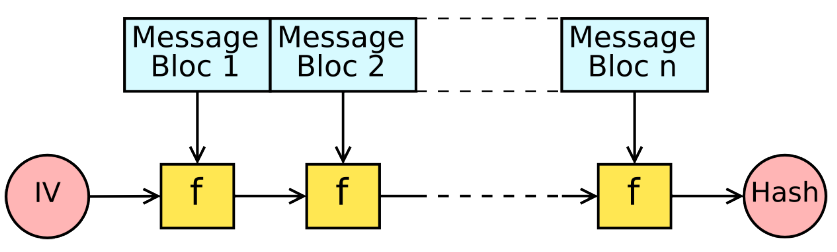
\includegraphics[width=0.3\textwidth]{img/merkle_damgard.png}
\end{center}

\paragraph*{Construction de Davies-Meyer}

La construction de Davies-Meyer permet de transformer un algorithme de chiffrement par bloc en une fonction de compression.

\begin{center}
    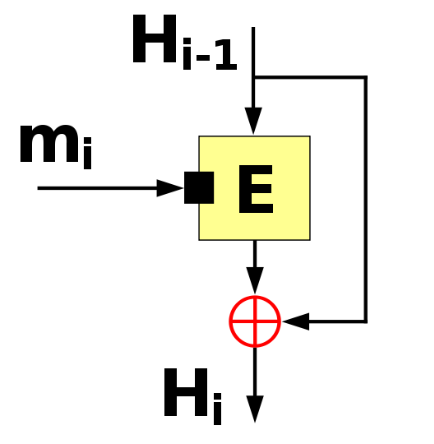
\includegraphics[width=0.15\textwidth]{img/davies_meyer.png}
\end{center}

\paragraph*{Quelques fonctions de hachage}

\begin{description}
    \item[MD5] : Empreintes de 128 bits, \textbf{cassée ! } Il est théoriquement possible de trouver des collisions en quelques secondes
    \item[SHA-1] : Empreintes de 160 bits, \textbf{cassée ! } Il théoriquement possible de trouver des collisions en environ $2^64$ opérations
    \item[SHA-256, SHA-512] : Empreintes de 256 et 512 bits et "sûre"
    \item[SHA-3] : Empreintes de 256 et 512 bits, similaire à AES
\end{description}

\paragraph*{Authentification symétrique}

La cryptographie symétrique peut garantir l’authenticité d’un canal de communication

une famille de fonction est définis comme $h_k:\{0,1\}* \times \kappa \longrightarrow \{0,1\}^l$. A éviter : $SHA256(X) \oplus K$. Exemple de familles sûre : HMAC, CBC-MAC,...

\paragraph*{Protocole : }
\begin{enumerate}
    \item Alice et Bob partage un secret $K$
    \item Alice envoie la liste $X$ ainsi que la valeur de MAC $\tau = h_k(X)$ à Bob
    \item Bob calcule $\tau = h_k(X')$ avec le message $X'$ reçu, et l'accepte comme étant authentique $\Longleftrightarrow \tau = \tau'$ où $\tau'$ est la valeur du MAC attaché au message.
\end{enumerate}

\paragraph*{HMAC}

Construit un MAC à partir de n’importe quelle fonction de hachage cryptographiquement sûre, HMAC\-MD5 et HMAC-SHA1 sont très largement utilisées en pratique (TLS, IPSec, ...).

\begin{align*}
& \text{Fonction de hachage } H \\
& \text{Clef secrète } K \\
& \text{Message à authentifier } X \\
& \text{Constantes } opad = 0x5c5c5c...5c \ ipad = 0x363636363...36 \\
& \\
& HMAC_k(X) = H((K\oplus opad)||H((K\oplus ipad)||X))
\end{align*}

\paragraph*{CBC-MAC}

Seulement sûr pour des messages de taille fixe !

\begin{center}
    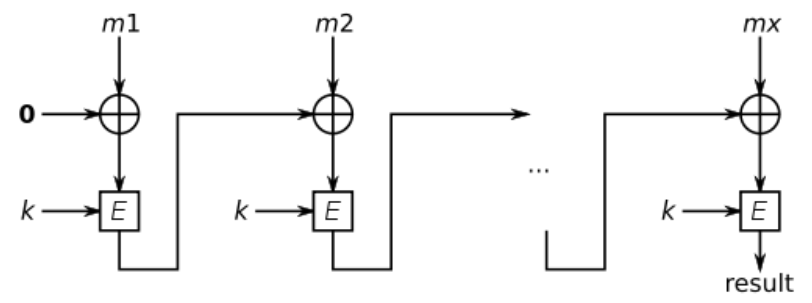
\includegraphics[width=0.4\textwidth]{img/cbc_mac.png}
\end{center}

\paragraph*{Protocole d'identification :} un mot de passe et un username permet d'identifier un uti\-lisateur.

\paragraph*{Protocole d'authentification :} e-banking, authentification via un certificat et le protocole TLS.

Il existe trois type d'authentification:
\begin{itemize}
    \item authentification faible
    \item authentification forte
    \item authentification "zero knowledge"
\end{itemize}

Un mot de passe est une authentification faible (si mdp espionné -> "\textbf{replay attack}").

Challenge-response est une authentification forte:
\begin{enumerate}
    \item Alice et Bob partage un secret symétrique commun
    \item Alice s'annonce auprès du serveur
    \item Bob génère un challenge $R$ (valeur aléatoire) à usage unique, stocke la pair $("Alice",R)$ et envoie $R$ à Alice.
    \item Alice calcule $\tau = MAC_K("Alice"||R)$ et envoie la pair ("Alice",$\tau$) à Bob.
    \item Bob reçoit la pair $(X,\tau')$, récupère le secret $K$ ainsi que la valeur $R$ correspondant à l'identité $X$, et calcule $\tau = MAC_K(X||R)$.
    \item Si $\tau=\tau'$ alors Bob considère que Alice s'est authentifié avec succès.
\end{enumerate}

\paragraph*{Protocole de Diffie-Hellman :}

Le but de ce protocole est de \textbf{partagé un secret} entre deux entités au moyen d'un canal non-confidentiel. Par contre, le canal doit être authentique ("man in the middle attack"). L'idée principale consiste à utiliser une fonction à sens unique.

\paragraph*{Logarithme discret}
\begin{align*}
& p = 2q + 1 \text{, $p$ est premier et $q$ en général est premier}\\
& g \in G \rightarrow \mathbb{Z}^*_p \\
& f : x \mapsto g^x \\
& x \longrightarrow y = g^x \mod p
\end{align*}

Protocole de Diffie-Hellman :
\begin{enumerate}
    \item Choisir $\mathbb{Z}^*_p$ et $g$ générateur de $\mathbb{Z}^*_p$
    \item Alice génère une valeur $a$ tel que $a\in\{1,2,...,p-2\}$, calcule $y_a=g^a\mod p$ et envoie $y_a$ à Bob
    \item Bob génère une valeur $b$ tel que $b\in\{1,2,...,p-2\}$,  calcule $y_b=g^b\mod p$ et envoie $y_b$ à Alice
    \item Alice calcule $k=y^a_b\mod p$ et Bob calcule $k=y^b_a \mod p$
    \item La clef secrète partagée est $k$.
\end{enumerate}

\paragraph*{Chiffrement RSA :}

L'idée est d'utiliser une fonction à sens unique munie d'une trappe.

\paragraph*{Génération de clef RSA :}
\begin{align*}
& \text{On définis $P$ comme l'ensemble des nombres premiers} \\
& p \in P \ q \in P \\
& n = pq \\
& \text{On définis l'opérateur $\oplus$ comme étant $e \oplus d$ : $e$ est premier avec $d$}\\
& e \oplus \phi(n) \\
& \phi(n) = (p-1)(q-1)\\
& d = e^{-1} \mod \phi(n)\\
& (n,e) \text{ : clef publique}\\
& (n,d) \text{ : clef privée}
\end{align*}

\paragraph*{Utilisation :} on chiffre un message $m$ avec $c=m^e\mod n$, on déchiffre avec $m =c^d\mod n$

\paragraph*{Signature RSA :}

Étant données la clef privée $(n,d)$ et un message $m$ à signer, on obtient la signature $s$ en calculant $s=m^d\mod n$. Étant donnés la clef publique $(n,e)$ et un message $m'$ muni d'une signature $s$, on vérifie la signature en calculant $m=s^e\mod n$ et on accepte la signature si et seulement si $m=m'$.

En pratique, on ne signe pas un message mais une empreinte $h$ de ce message : $h=H(m)$ où $H(.)$ est une fonction de hachage cryptographiquement sûr. Étant donné deux signatures $s=m^d\mod n$ et $s=m'^d\mod n$ on peut créer une nouvelle signature :
$$
s \cdot s' \equiv m^d \cdot m'^d \equiv (m\cdot m')^d \mod n 
$$

\paragraph*{Signature RSA rapides :}

\begin{enumerate}
    \item On calcule $d_p=d\mod (p-1)$, ainsi que $d_q=d\mod (q-1)$
    \item On calcule $q^{-1}\mod p$ et $p^{-1}\mod q$ via Euclide étendu
    \item Signature partielle :
    \begin{itemize}
        \item $s_p = m^{d_p} \mod p$
        \item $s_q = m^{d_q} \mod q$
    \end{itemize}
    \item Signature finale : $s=(s_p(q^{-1} \mod p)q+s_q(p^{-1} \mod q)p) \mod n$
    \end{enumerate}

\paragraph*{Signature d'El-Gamal :}

Repose sur la difficulté de résoudre le problème du logarithme discret.

\begin{itemize}
    \item On génère un nombre premier $p=2q+1$ et un générateur $g\in \mathbb{Z}^*_p$
    \item On génère $a \in \{1,...,p-2\}$
    \item On calcule $A=g^a\mod p$
    \item Clef publique : $(p,g,A)$
    \item Clef privé : $(p,g,a)$
\end{itemize}

\paragraph*{Signature :}

On utilise une fonction de hachage cryptographiquement sûre $h:\{0,1\}^* \longrightarrow \{1,...,p-2\}$. On calcule un nombre $k\in\{1,...,p-2\}$ premier avec $p-1$. pour signer un message $m$, on calcule $r=g^k\mod p$ ainsi que $s=k^{-1}(h(m)-ar)\mod p-1$. La signature du message est $(r,s)$.

\paragraph**{Vérification : } $r\in{1,...,p-2}$ et $A^rr^s\equiv g^{h(m) \mod p}$

\paragraph*{Choix de la taille des clés :} Difficile de choisir les paramètres cryptographiques. 1ère chose à prendre en compte : la difficulté supposée de casse un problème difficile ($n=pq$, ou logarithme discret).

\paragraph*{Nombres premiers :} Pour trouver un nombre premier de grande taille : générer un nombre impair aléatoire, tester si il est bon sinon recommencer, tester si il convient à l'algorithme sinon recommencer. En moyenne : $\ln(p)$ fois pour obtenir un nombre.

\paragraph*{Test de Fermat :} utiliser le petit théorème de Fermat pour tester le nombre si premier ou non (problème avec les nombres de Carmichael (infinité de nombre !)).

\paragraph*{Test de Miller-Rabin :} soit $n$ un nombre entier et $n\geq 3$ et $k$ un paramètre de sécurité :
\begin{itemize}
    \item écrire $n-1=2^sd$ avec $d$ impair
    \begin{itemize}
        \item générer un nombre $a$ entre $1$ et $n-1$ (compris)
        \item calculer $x=a^d\mod n$, si $x\equiv1\mod n$ ou $x\equiv n-1 \mod n$ continue;
        \item Pour $1 \leq r \leq s-1$, calculer $x_r \leftarrow x^2_{r-1}\mod n$, avec $x_0=a^d\mod n$. Si $a^{2^rd}$ n'est pas congrue à $-1 \mod n$ pour $1 \leq r \leq s-1$, alors $n$ n'est pas premier et stopper. Sinon, continuer. 
    \end{itemize}
    \item $n$ est probablement premier.
\end{itemize}

La probabilité que le test de Miller-Rabin annonce $n$ comme étant premier de manière erronnée est inférieure à $4^{-k}$.

\paragraph*{Exponentiation rapide :} crucial de calculer $a^b\mod c$ rapidement. On a donc $a^b \equiv (a^{b_0})^{2^0}(a^{b_1})^{2^1}(a^{b_2})^{2^2}...(a^{b_{n-1}})^{2^{n-1}}$. Par exemple, pour $b= 37 = 100101$ on a donc : $a^b \equiv (a^1)^{2^0} (a^0)^{2^1} (a^1)^{2^2} (a^0)^{2^3} (a^0)^{2^4} (a^1)^{2^5} \mod c$. On écrit les nombres de droite à gauche (on commence par le bit de poid faible).

\paragraph*{Courbes elliptiques :} une courbe elliptique $C$ définie sur $\f$ avec les coefficients $a,b\in\f$ est définie comme étant l'ensemble des points $(x,y)\in\f^2$ qui satisfont l'équation suivante dans $\f[x]$: $y^2=x^3+ax+b$ et on a en plus un point $O$ appelé \textbf{point à l'infini}.

\paragraph*{Addition de points :} soit $P=(x_1,y_1),Q=(x_2,y_2)$ sur une courbe elliptique avec $x_1\neq x_2$, on calcule $R=(x_3,y_3)=P+Q$: $x_3=(\frac{y_2-y_1}{x_2-x_1})^2-x_1-x_2$ et $y_3=-y_1+(\frac{y_2-y_1}{x_2-x_1})(x_1-x_3)$.

\paragraph*{Doublement des points :} soit $P=(x_1,y_1)$ sur une courbe elliptique, on calcule on calcule $R=(x_2,y_2)=2P$ : $x_3=(\frac{3x^2_1-1}{2y_1})^2-2x_1$ et $y_3=(\frac{3x^2_1-1}{2y_1})(x_1-x_2)-y_1$.

\paragraph*{Courbes elliptiques sur $GF(2^r)$ :} 
\begin{itemize}
    \item $y^2+b_1y=x^3+a_1x+a_0$ avec $b_1\neq0$
    \item $y^2+xy=x^3+a_2x^2+a_0$ avec $a_0\neq0$
\end{itemize}

\paragraph*{Théorème de Hasse :} Le théorème de Hasse garantie que n’importe quelle courbe elliptique définie sur un corps suffisament grand aura un grand nombre de points. Si $N$ est le nombre de points sur une courbe elliptique définie sur un
corps fini à $q$ éléments, alors $N$ est borné par $|N-(q+1)\leq 2\sqrt{q}|$.

\paragraph*{Courbes Elliptiques et Extensions de Corps :} Une courbe elliptique est dite être définie sur le corps fini $GF(q)$ avec $q=p^n$ pour un entier naturel $n$ si ses coefficients sont dans $GF(q)$.La courbe définie par toutes les solutions dans l'extension de corps $GF(q^r)$ est noté $E_r$. Soit $s=q+1-N$. On note $\alpha$ et $\beta$ les deux racines du polynôme caractéristique $T^2-sT+q$ d'une courbe elliptique $E$. Pour une courbe elliptique $E$ définie sur $GF(q)$, le nombre $N_r$ de points qu'elle possède lorsqu'elle est définie sur $GF(q^r)$ avec $r \geq 1$ est donnée par $N_r=-\alpha^r-\beta^r+q^r+1$.

\paragraph*{Avantages des courbes elliptiques :}
\begin{itemize}
    \item Le problème du logarithme discret est transposable à une courbe elliptique
    \item Les algo efficace pour le logarithme discret dans $GF(q^n)$ ne sont pas applicable aux courbes
    \item Les courbes elliptiques définis sur $GF(2^n)$ sont efficacement implémenté en hardware
\end{itemize}

\paragraph*{ECDH :} Le protocole de Diffie-Hellman peut être implémenté sur le
groupe des points d’une courbe elliptique :
\begin{enumerate}
    \item Se mettre d’accord sur une courbe elliptique cryptographiquement sûre et sur un point $G$ d’ordre $n$. Le nombre $h = N/n$ est appelé le co-facteur et devrait être petit, de préférence égal à $1$.
    \item Alice génère une valeur secrète $a \in \{1,...,n-1\}$ uniformément au hasard, calcule $Y_a = aG$, et envoie $Y_a$ à Bob via le canal authentique.
    \item Bob génère une valeur secrète $b \in \{1,...,n-1\}$ uniformément au hasard, calcule $Y_b=bG$, et envoie $Y_b$ à Alice via le canal authentique.
    \item Alice calcule $K=aY_b$ et Bob $K=bY_a$.
    \item La clé secrète partagée est $K$.
\end{enumerate}

\paragraph*{El-Gamal :}
\begin{enumerate}
    \item Se mettre d'accord sur une courbe elliptique cryptographiquement sûre et sur un point $G$ d'ordre $n$.
    \item Clé privé : $a\in\{1,...,n-1\}$
    \item Clé publique : $aG$
    \item Pour chiffrer un message $M$, on génère un nombre $k\in\{1,...,n-1\}$ secret.
    \item Le texte chiffré est la pair $(kG,M+k(aG))$
    \item Pour déchiffrer, on calcule $a(kG)$ puis $M+k(aG)-a(kG)=M$
\end{enumerate}

\end{document}